\section{Modellierung der Asynchronmaschine}
Dieser Abschnitt befasst sich mit der Benutzung der beigefügten Simulation. Es soll beschrieben werden welche Parameter angepasst werden können. Es sollen weiterhin verschiedene Simulationen dargestellt werden um darzustellen wie sich ein richtig eingestellter Motor verhalten sollte.
Die Modellierung wurde in drei Abschnitte unterteilt.
\begin{itemize}
	\item Feldorientierte Regelung
	\item Transformation
	\item Motormodell
\end{itemize}
\subsection{Konfiguration des Motormodells}
Dieses Modell kann grundsätzlich an jeden Asynchronmotor angepasst werden. Es muss dabei nur beachtet werden, dass alle Parameter im \textit{Model Explorer} richtig eingestellt werden.
Es folgt nun eine Auflistung von Motorparametern, welche bekannt sein müssen.\\\par

	\begin{tabular}{c|l|c}
	Bezeichnung & Beschreibung & \textit{Model Explorer} \\ \hline
	\multicolumn{3}{c}{Elektrische Kenngrößen}\\ \hline
	\begin{math} I_{\mu}^{+} \end{math} & Magnetisierungsstrom & I\_magnet\\
	\begin{math} \Psi_{R}^{+} \end{math} & Läuferfluss & PsiR\_plus\\
	\begin{math} L_{R}^{+} \end{math} & Läuferinduktivität & I\_magnet\\
	\begin{math} L_{\sigma}^{+} \end{math} & Streuinduktivität & Lsigma\_plus\\
	\begin{math} R_{R}^{+} \end{math} & Läuferwiderstand & RR\_plus\\
	\begin{math} R_{S} \end{math} & Ständerwiderstand & Rs\\
	\begin{math} I_{A} \end{math} & Start-Strom & StartStrom\\
	\begin{math} M_{A} \end{math} & Start-Moment & StartMoment\\
	\begin{math} p \end{math} & Polpaaranzahl & p\\
	\multicolumn{3}{c}{Mechanische Kenngrößen}\\ \hline
	\begin{math} \mu \end{math} & Reibungskoeffizient & Rreib\\
	J & Trägheitsmoment & J\\
	\end{tabular}\\\par
	
Diese Parameter müssen in den \textit{Model Explorer} eingetragen werden. Fehlt einer oder mehrere Parameter kann es passieren, dass das Model kaum oder garnicht funktioniert, also sich nicht wie erwartet verhält.\\\par
	
Um nun eine Simulation sinnvoll durchzuführen, müssen noch Sollvorgaben und Lastsituationen eingetragen werden. Dafür können die die Blöcke Drezahlvorgabe und Lastvorgabe genutzt werden. Diese Blöcke verwenden die Parameter MLast und wSoll, diese sollten ebenfalls an realistische Last-Situationen angepasst werden.\\\par

\subsubsection{Bestimmung von dem Reibungskoeffizienten $\mu$}
Sollte $\mu$  nicht bekannt sein, lässt sich dieser leicht über die Simulation ermitteln. Dafür sind folgende Schritte notwendig.
\paragraph{Anpassung der Simulation}
	Im ersten Schritt muss der Momentregler vom Rest der Simulation getrennt werden und durch das konstante Nennmoment ersetzt werden, dies ist in in \autoref{fig:rreibComp} zu sehen.
	\begin{figure}[H]
		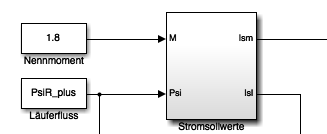
\includegraphics[width=2.5in]{pictures/Reibkoeffizient_bestimmen}
		\caption{Aufbau der Simulation zur Bestimmung des Reibkoeffizient}
		\label{fig:rreibComp}
	\end{figure}
\paragraph{Bestimmung des Parameters}\label{par:mu0BestimmungParameter}
	Nun muss \begin{math}\mu\end{math} solange verändert werden, bis die Drehzahl gleich der Nenndrehzahl wird. Dabei müssen alle MLast gleich null sein. Dies ist im \textit{Model Explorer} einzustellen. In \autoref{fig:rreibChart} ist Beispielhaft zu erkennen, wie sich die Drehzahl der Nenndrehzahl nähert. 
	\begin{figure}[H]
		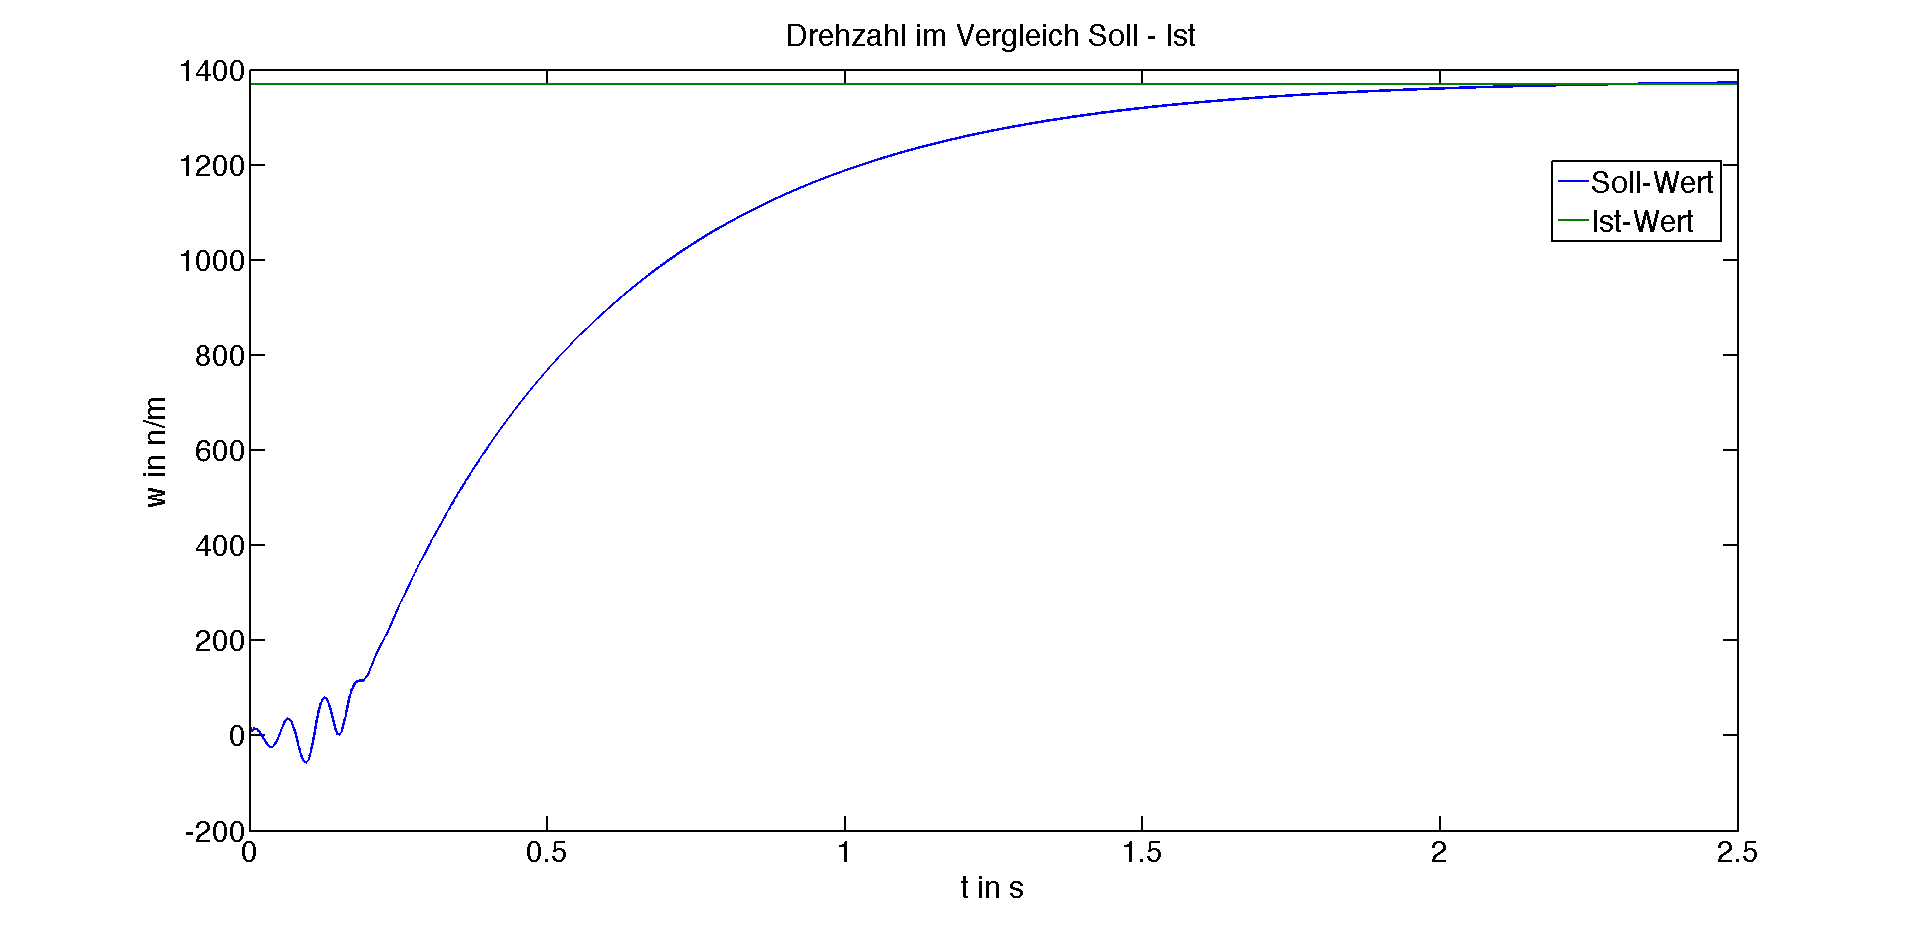
\includegraphics[width=0.5\textwidth]{pictures/Reibkoeffizient_Chart.png}
		\caption{Zeitlicher Verlauf der Drehzahl im Vergleich zur Nenndrehzahl(hier Solldrehzahl)}
		\label{fig:rreibChart}
	\end{figure}	
	
\subsection{Simulation der Asynchronmaschine}
Im folgenden sollen verschiedene Simulations-Szenarien dargestellt und erläutert werden.
\subsubsection{Sollwertvorgabe - ohne Last}
Dieses Szenario kann genutzt werden um die grundsätzliche Funktion des Modell sicherzustellen.
\paragraph{Einstellung der Parameter}
Im ersten Schritt müssen alle MLast Parameter auf 0 gesetzt werden(siehe \ref{par:mu0BestimmungParameter}). Außerdem sollten sinnvolle WSoll Vorgaben gemacht werden, so könnte zum Beispiel folgender Ablauf gewählt werden:\\\par
	\begin{center}
		\begin{tabular}{c|c}
			Zeitpunkt t & Solldrehzahl $n_{Soll}$ in n/min\\ \hline
			1s & 500 \\
			6s & 1370 \\
		\end{tabular}
	\end{center}
\paragraph{Durchführung der Simulation}
Im nächsten Schritt sollte eine sinnvolle Zeit für die Simulation gewählt werden. In diesem Beispiel haben wir 10s gewählt.
\paragraph{Analyse der Ergebnisse}
	In \autoref{fig:KeineLastMoment} ist zu sehen, dass der Motor auf Vorgabeänderungen der Drehzahl mit starken Schwankungen des Drehmomentes reagiert.\\
	Bei einer Erhöhung der Drehzahl wird der Motor versuchen das Drehmoment innerhalb seiner Grenzen(Strom, Spannung, etc.) zu erhöhen um die gewünschte Drehzahl zu erreichen. Bei einer Überschreitung wird er ruckartig das Moment verringern.\\
	Bei einer Verringerung der Drehzahl reagiert der Motor damit, das Moment zu verringern, dort ist zu sehen wie der Moment des Motors negativ wird, da dem Motor fast keine Energie mehr zugeführt wird und damit auch kein Antrieb im Motor steckt.
	\begin{figure}[H]
		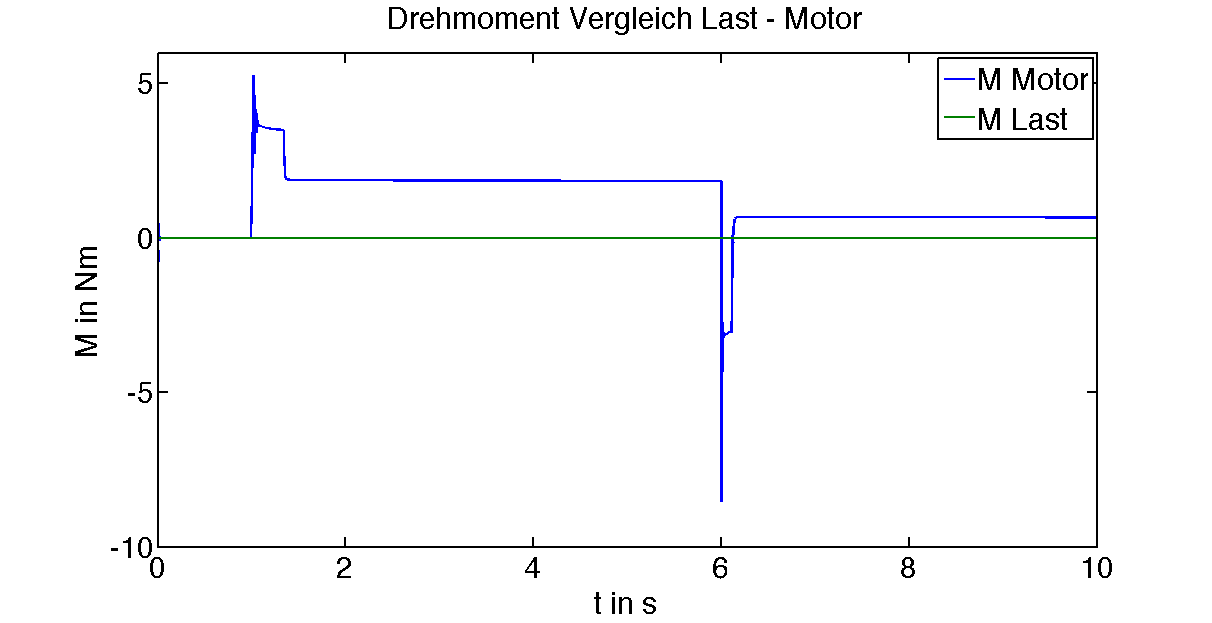
\includegraphics[width=0.5\textwidth]{pictures/KeineLastMoment.png}
		\caption{Zeitlicher Verlauf des Drehmomentes}
		\label{fig:KeineLastMoment}
	\end{figure}	
	In \autoref{fig:KeineLastDrehzahl} sind keine Besonderheiten zu erkennen, der Motor versucht nach seinen Möglichkeiten der Vorgabe zu folgen und schafft dies in einer relativ kurzen Zeit.
	\begin{figure}[H]
		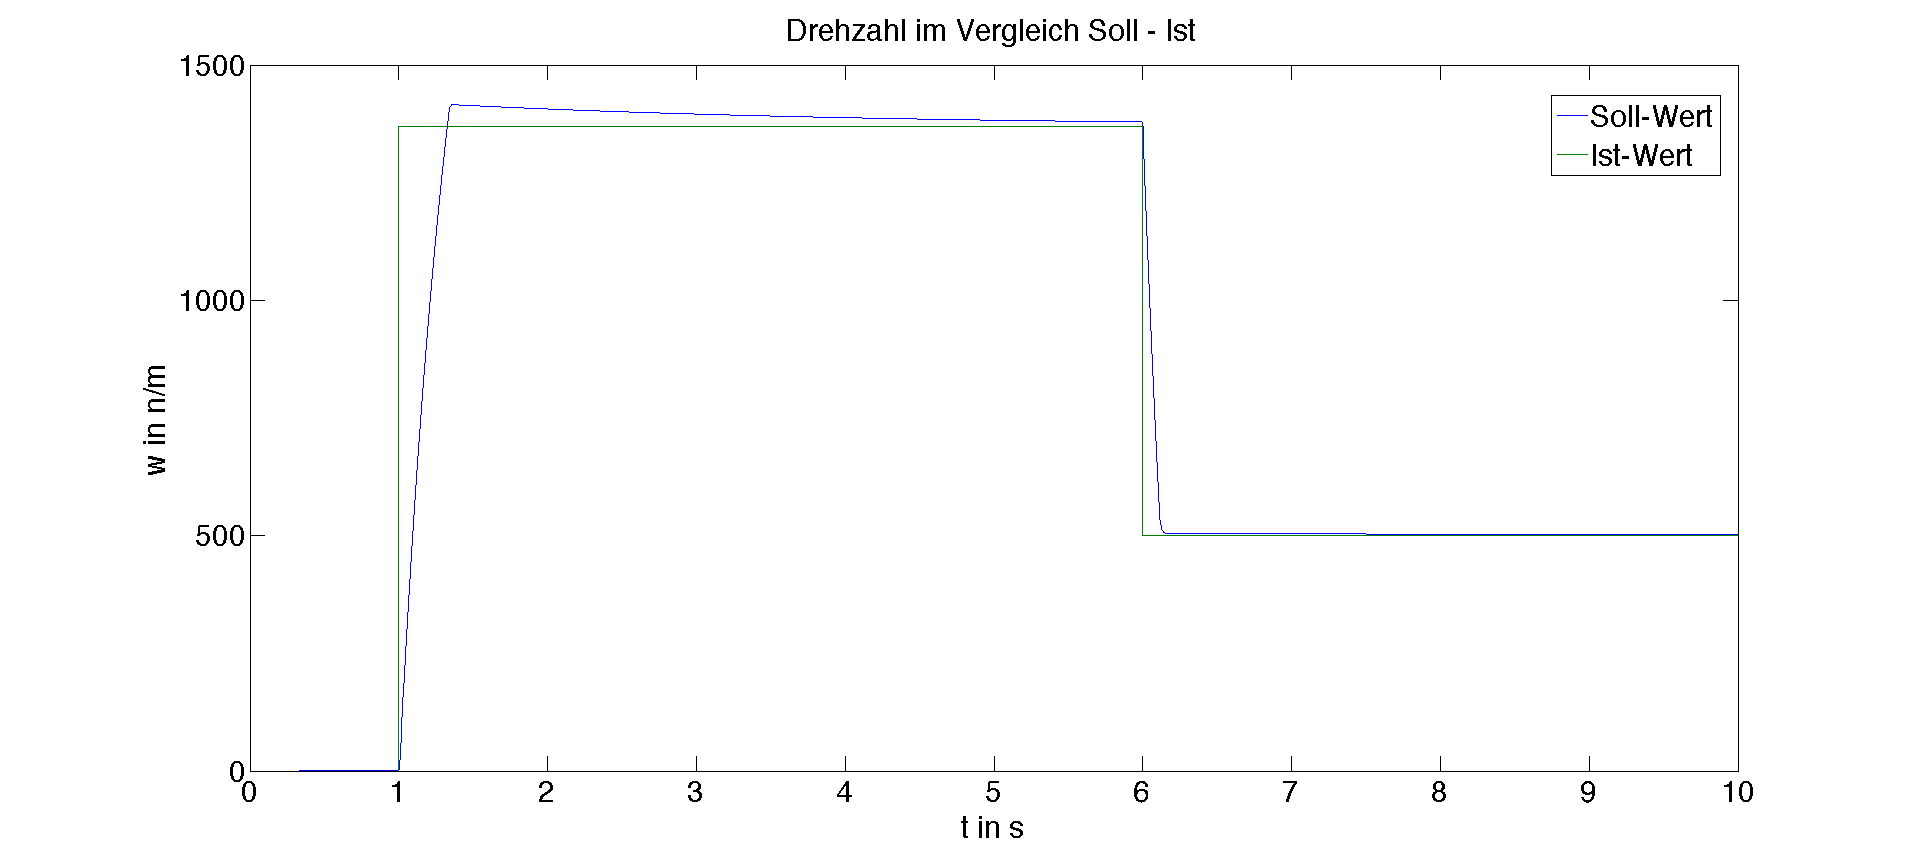
\includegraphics[width=0.5\textwidth]{pictures/KeineLastDrehzahl.png}
		\caption{Zeitlicher Verlauf der Drehzahl}
		\label{fig:KeineLastDrehzahl}
	\end{figure}	
\subsubsection{Sollwertvorgabe - mit Last}
Diese Simulation zeigt das Lastverhalten des Motors. Es soll gezeigt werden, dass dieser bei seinem angegebenen Haltemoment stehen bleibt und bei zu großer Last sogar rückwärts dreht.
\paragraph{Einstellung der Parameter}
	Für diese Simulation sollten sinnvolle Werte gewählt werden. In unserem Fall wurden die Werte so gewählt, dass im ersten Zeitfenster(1s-6s) zu sehen ist wie die Maschine durch eine Last gehalten wird und im zweiten Zeitfenster(6s-10s) zu sehen ist wie die Last die Maschine dreht.\\\par
	\begin{center}
		\begin{tabular}{c|c|c}
			Zeitpunkt t & $n_{Soll}$ in n/min & M in Nm\\ \hline
			1s & 1370 & 3,8\\
			6s & 500 & 10\\
		\end{tabular}
	\end{center}
\paragraph{Analyse der Ergebnisse}
	In \autoref{fig:LastMoment} is zu sehen, dass das Drehmoment des Motors und der Drehmoment der Last sich angleichen, da der Motor versucht die eingestellte Drehzahl zu erreichen. Ab Sekunde 6 ist zu sehen, dass das Drehmoment des Motors deutlich unter dem der Last ist. 
	Auch wenn der Motor im ersten Moment versucht, gegen die Last anzukommen bringt ihn dann die simulierte Begrenzung des Stromes wieder auf sein Haltemoment.
	\begin{figure}[H]
		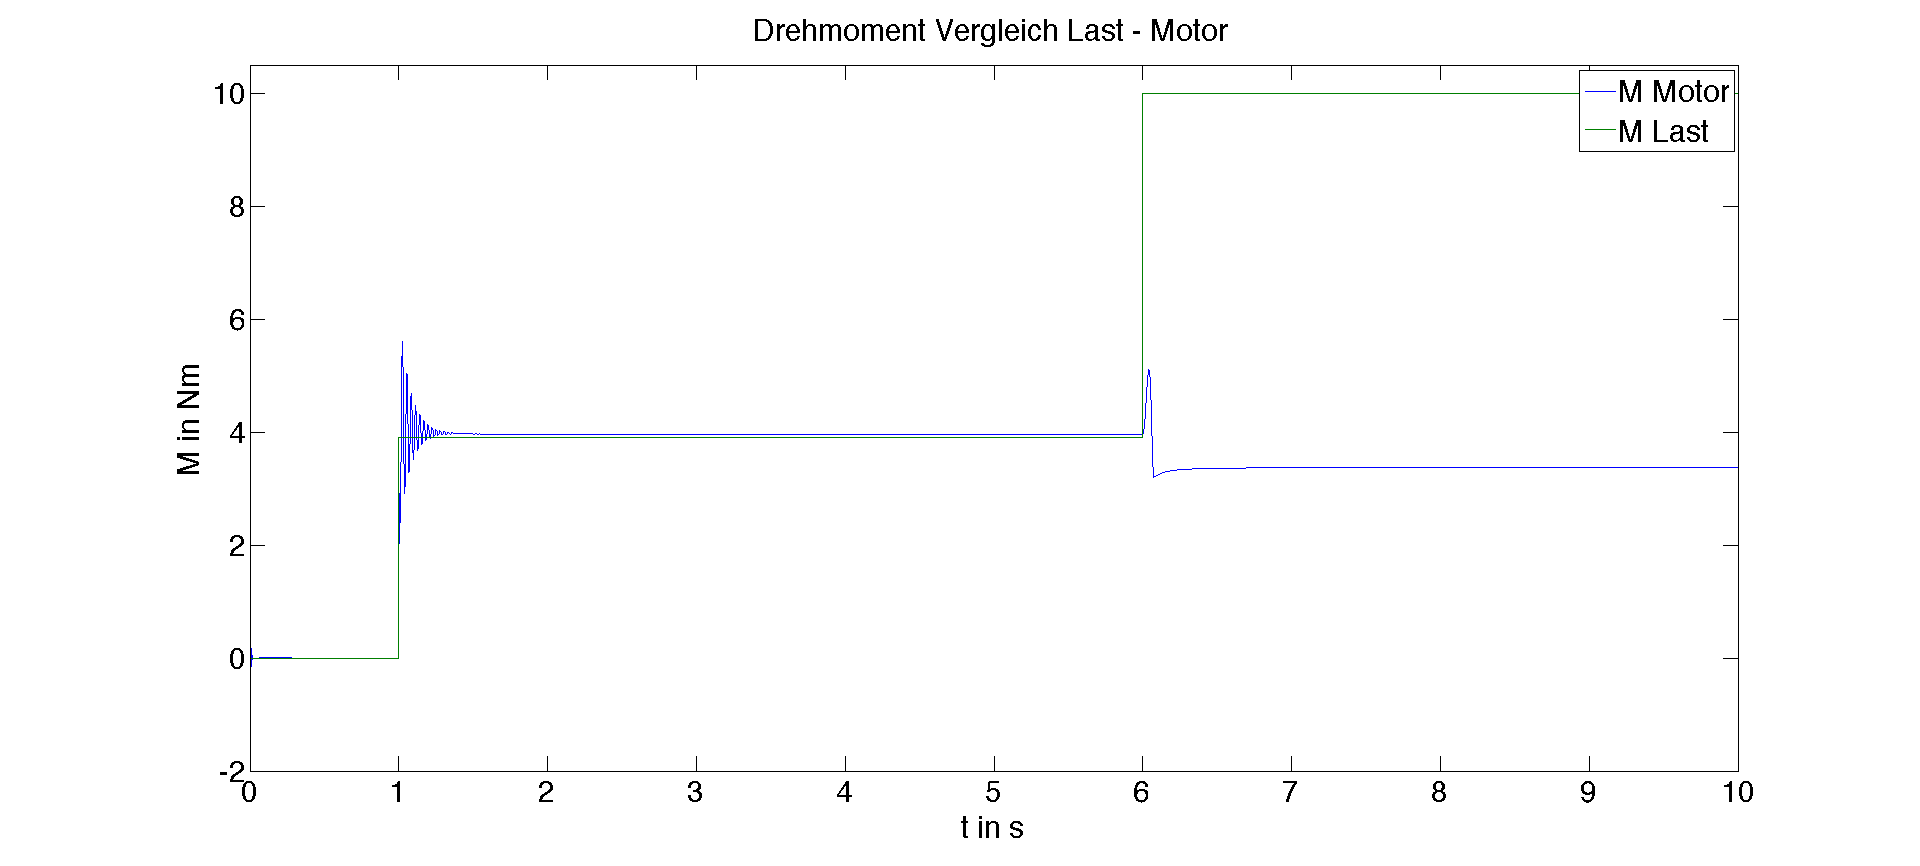
\includegraphics[width=0.5\textwidth]{pictures/LastMoment.png}
		\caption{Zeitlicher Verlauf des Drehmomentes}
		\label{fig:LastMoment}
	\end{figure}
	Einen passenden Verlauf können wir in \autoref{fig:LastDrehzahl} sehen. Im Zeitraum von 1s - 6s ist zu sehen, wie der Motor nahezu steht. Sobald dann ab Sekunde 6 das Moment der Last größer als sein Haltemoment wird, fängt der Motor an, sich rückwärts zu drehen.
	\begin{figure}[H]
		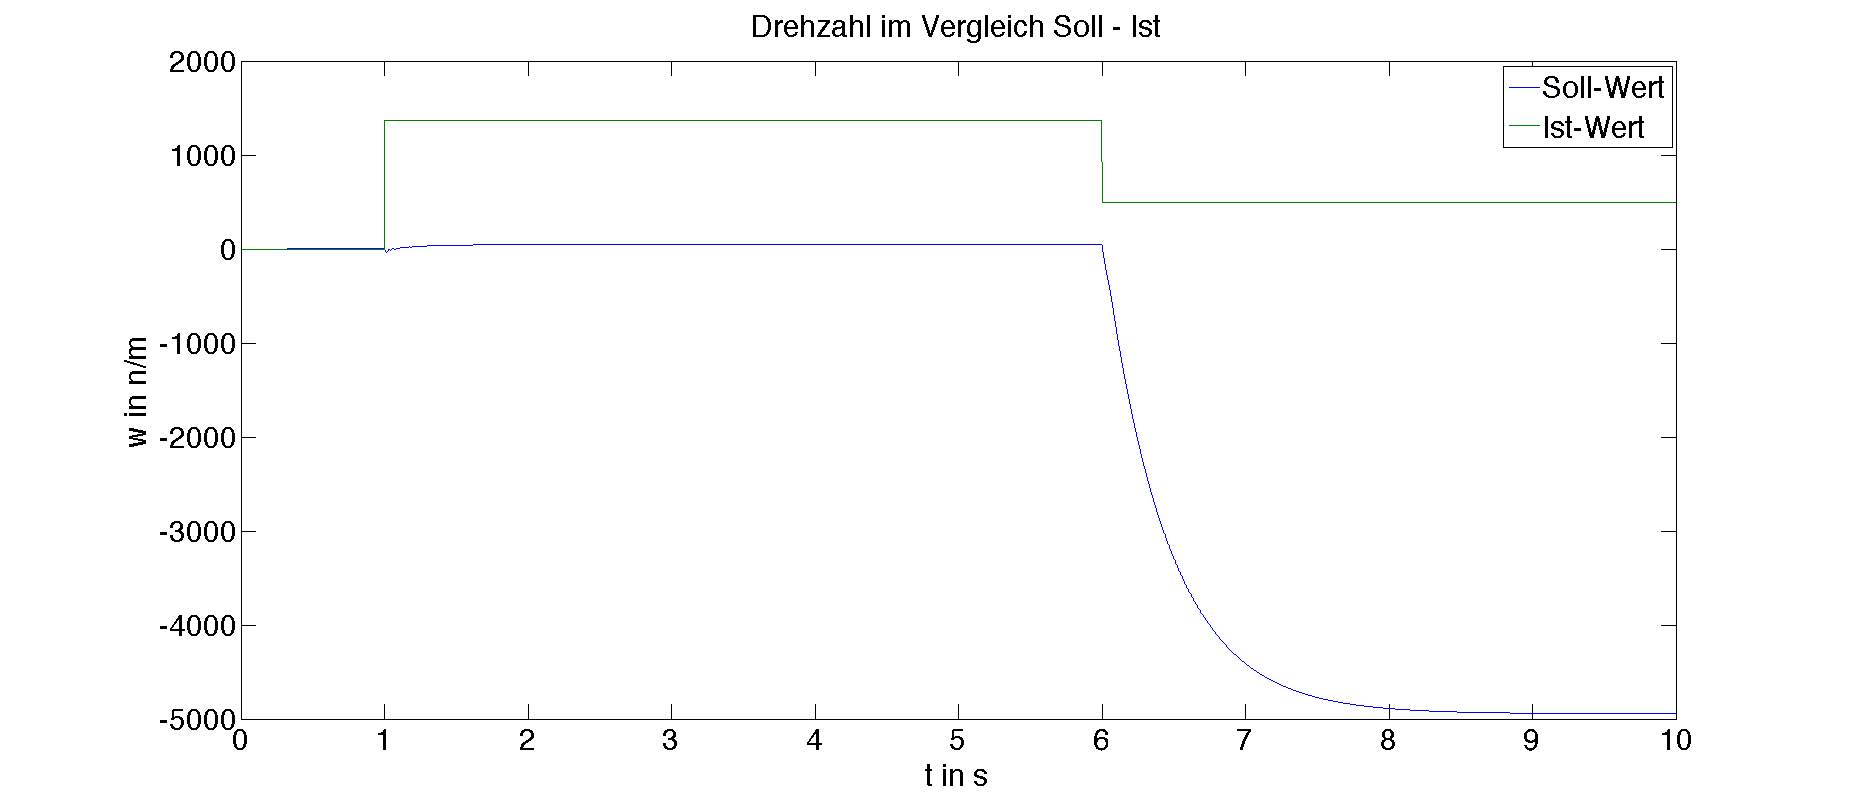
\includegraphics[width=0.5\textwidth]{pictures/LastDrehzahl.png}
		\caption{Zeitlicher Verlauf der Drehzahl}
		\label{fig:LastDrehzahl}
	\end{figure}
\subsection{Schwächen des Modells}
Dieses Modell stellt keine reale Abbildung des Motors dar, kann aber einen Eindruck vermitteln, welches Verhalten von diesem Asynchronmotor zu erwarten ist.\\
Vor allem in der Begrenzung von Strom und Spannung ist deutliches Verbesserungspotential zu sehen.\\
So wird die Spannung im gesamten Modell nicht begrenzt und steigt teilweise auf bis zu 1500V, dies ist mit einer Versorgungsspannung von 230V-AC aber nicht möglich. Änderungen dieser Parameter können an den Reglerbausteinen vorgenommen werden, dies führt allerdings zu einer Neueinstellung der Parameter.\\ Es ist zu erwarten, dass der Motor nicht ganz so schnell reagieren kann.